% !TeX root = ../FinalRepordCS.tex

\chapter{Introduction}

\section{Background}

Network security is a recent scorching topic and affects everyone's vital interests. Mature PKI-based password management systems such as SSL and TLS are regarded as an excellent way to solve the problem of encrypted communication in computer networks. However, in the field of the Internet of Things, due to issues such as node computing performance and the difficulties in key management in large amount of nodes, PKI systems are not suitable in it. 

According to Gartner\cite{gartnerresearchiot}, there will be over 43 billion IoT devices connected to the internet by 2023, and the IoT market size will reach US\$1.4 trillion. The rapid development of the IoT is mainly due to the following trends. Also, the MIIT suggests that the IoT is a future development trend that will have a profound impact on all industries\cite{iot13th5yr}. The security of the communication channel in the Internet of Things is of utmost importance, given the critical role of IoT. Ensuring the security of IoT communication channels will be a highly significant and crucial subject.

To address this problem, and based on previous research, some physical layer key generation methods have been proposed. Physical layer key generation is a technique for generating cryptographic keys from the physical characteristics of a wireless communication channel. This can be done by exploiting the unique features of the channel, such as its fading characteristics, noise properties, and path loss. Physical layer key generation is particularly attractive for wireless sensor networks (WSNs) because it does not require any prior shared information between the nodes, and it can be implemented with relatively low computational overhead.

Physical layer key generation has recently been a research hotspot in academia and industry\cite{7120014}. However, existing research often focuses only on traditional wireless communication technologies such as Wi-Fi, ZigBee, and 5G Radio Access Network. While in the area of Low-Power Wide-Area Networks (LPWAN)\cite{iotfactorylpwan}, the long communication distance, low power consumption, and low transmission rate bring new research challenges to physical layer key generation.
\begin{figure}
  \centering
  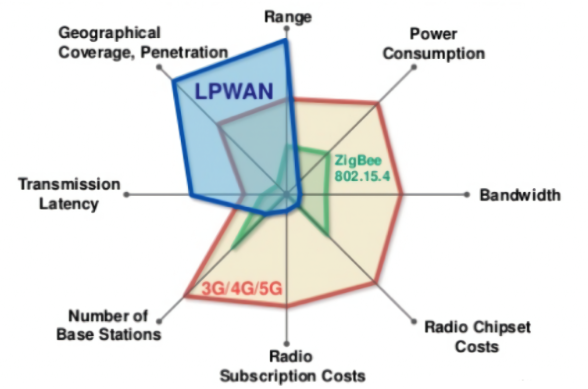
\includegraphics[width=0.6\linewidth]{fig1-1.png}
  \caption{LPWAN vs. Other wireless communication technologies\cite{iotfactorylpwan}}
  \label{fig:1-1}
\end{figure}
LoRa, a widely used LPWAN communication technology, is a physical layer modulation method defined by Semtech Corporation and based on the Chirp spread spectrum technology, which achieves a reception sensitivity of -148 dBm, a small data rate (0.3-50kbps) in exchange for a high communication range (3km in urban areas and 15km in suburban areas) and low power consumption (battery-powered operation for up to 10 years under certain conditions)\cite{lorawanpara}. It provides a reliable connectivity solution for low-power IoT devices, especially for communication or data interaction with outdoor wireless sensor networks.
\begin{figure}
  \centering
  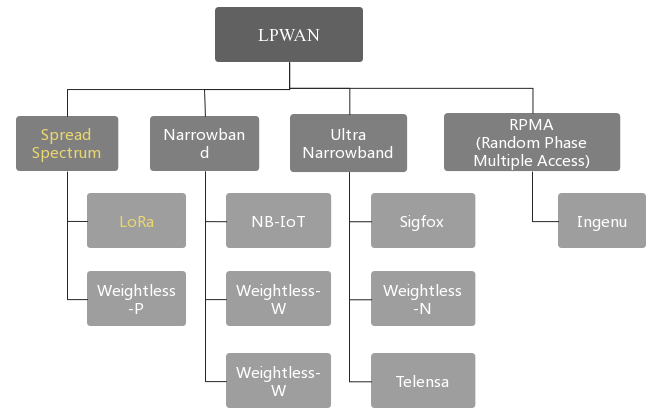
\includegraphics[width=0.8\linewidth]{fig1-2.png}
  \caption{LPWAN Classification}
  \label{fig:1-2}
\end{figure}
Despite many advantages, the biggest problem is that physical layer encryption for LoRa is not well standardized. Because it is a type of wireless communication tech that has to broadcast its signal, it makes the communication information easy to capture and monitor. Thus, physical layer encryption for LoRa communication is a significant topic. 

In short, physical layer key generation for LoRa is still under development, but it can potentially revolutionize the security of LoRa-based networks. It can be used to secure a wide range of applications, including smart cities, industrial automation, and the Internet of Things.

\section{Objectives}

The specific research objectives are:

1. Understand the characteristics and limitations of LoRa communication technology, including its communication range, power consumption, data rate, and noise immunity.



2. Understand the different physical layer encryption algorithms and compare their advantages and disadvantages. Choose one as the basis for the implementation of this Guide Study, and find ways to improve it.

3. Select and configure suitable LoRa modules and development boards to realize the LoRa communication protocol stack and basic data transmission functions.

4. Implement a physical layer encryption algorithm for LoRa communication to protect the privacy and confidentiality of data. The algorithm should suit LoRa's low data rate and long communication distance characteristics and have strong anti-interference and anti-jamming capabilities.

5. Test and evaluate the performance of the encryption algorithm via multiple scenario experiments and simulations. Compare the performance with existing key generation algorithms for LoRa physical layer and analyze its pros and cons.

